\chapter{The Gradient, Directional Derivatives, and the Chain Rule}
\label{ch33:gradient-directional-chain-rule}

In the last chapter we learned to take a function of several variables, freeze
all but one of its inputs, and differentiate the survivor. That gave us the
partial derivatives $\pdv{f}{x}$ and $\pdv{f}{y}$: the slopes you feel if you
walk due east or due north across rolling terrain. They are exact answers, but to
only two questions. Real hills are not made of
north-south and east-west walks. A river runs diagonally. A ball rolls downhill
in whatever direction is steepest, which is almost never one of the axis
directions. If all we can ever ask is ``how steep is it if I head exactly east?''
we have not yet learned to read the surface beneath our feet.

This chapter asks: \emph{how fast does $f$ change if I walk in any direction I
choose?} The answer, for \emph{every} direction at once, is contained in a single
arrow, the \textbf{gradient} $\grad f$. It points in the direction of steepest
ascent. Its length tells you how steep that steepest climb is. And it is
perpendicular to the level curves (the contour lines) of $f$; Section~\ref{ch33:perp}
shows why. From there the multivariable chain rule becomes a short formula, and
linear approximation upgrades the tangent line to a tangent \emph{plane}.
\emph{Gradient descent}, the method used to train nearly every modern neural
network, becomes plain geometry: keep stepping in the direction of $-\grad f$ and
you walk downhill. The chapter ends with two ways to locate highest and lowest
points: a second-derivative test for surfaces, and a method for maximizing a
function when its inputs are tied together by an equation.

\chapterline

\section{Walking in an Arbitrary Direction}
\label{ch33:directional}

Stand on a hillside whose height above sea level is $f(x,y)$. You are at the
point $(a,b)$. The two partial derivatives answer only two of the infinitely many
walks you could take: $\pdv{f}{x}\big|_{(a,b)}$ is your rate of climb heading
east, $\pdv{f}{y}\big|_{(a,b)}$ heading north. Now suppose you want to set off in
some other direction -- say northeast, or exactly $30^\circ$ north of east. How
steep is the ground \emph{that} way?

To name a direction we need vectors, which we use from here on. A
\textbf{vector} in the plane is a pair of numbers $\vec v=(v_1,v_2)$, pictured as
an arrow that goes $v_1$ units east and $v_2$ units north; vectors are printed in
bold. Adding two vectors adds their entries, and multiplying by a number $t$
stretches the arrow: $t\vec v=(tv_1,tv_2)$. The \textbf{length} (or
\textbf{norm}) of $\vec v$ is $\norm{\vec v}=\sqrt{v_1^2+v_2^2}$, by Pythagoras.
A \textbf{unit vector} is a vector of length $1$; it records a direction and
nothing else. For example, $(3,4)$ has length $5$, and $\tfrac15(3,4)=(0.6,\,0.8)$
is the unit vector pointing the same way.

Name the direction of your walk with a unit vector
$\vec{u}=(u_1,u_2)$, $\norm{\vec u}=1$. Walking ``in direction $\vec u$''
starting from $(a,b)$ means tracing the straight path
\[
  (a,b) + t\,\vec u = (a + t u_1,\; b + t u_2), \qquad t \ge 0,
\]
where $t$ is the distance you have walked (because $\vec u$ has length one, $t$
\emph{is} arc length). Your height along this path is a function of the single
variable $t$:
\[
  g(t) = f(a + t u_1,\; b + t u_2).
\]
The slope of the ground in direction $\vec u$ is how fast your height changes per
unit distance walked, at the start of the walk: that is, $g'(0)$.

\begin{figure}[H]
\centering
\begin{tikzpicture}[scale=1.7]
% the (x,y) floor plane drawn schematically
\draw[gray!40] (-1.2,-1.3) -- (2.6,-1.3) -- (3.4,0.0) -- (-0.4,0.0) -- cycle;
\node[gray!80!black, font=\footnotesize, anchor=west] at (1.75,-1.12) {the $(x,y)$ plane};
% point (a,b)
\coordinate (ab) at (0.2,-0.7);
\fill[black] (ab) circle (0.8pt);
\node[below left, font=\small] at (ab) {$(a,b)$};
% the straight walk in the plane, and the direction u
\draw[gray!70] (ab) -- (1.3,-0.45);
\draw[-{Stealth[length=2.5mm]}, thick, sourceblue]
  (ab) -- ++(0.66,0.15) node[below right=-1pt, font=\small] {$\vec u$};
% heights above the walk
\draw[gray!60, densely dotted] (0.7,-0.586) -- (0.7,-0.106);
\draw[gray!60, densely dotted] (1.2,-0.472) -- (1.2,0.348);
\draw[gray!60, densely dotted] (1.3,-0.45) -- (1.3,0.42);
% the slice curve g(t) rising above the line
\draw[curveblue, very thick]
  plot[smooth, domain=0:2.2, samples=40]
  ({0.2+\x*0.5},{-0.7+\x*0.114 + 0.55*\x - 0.07*\x*\x});
\node[curveblue, font=\small, anchor=west] at (1.33,0.47) {$g(t)=f(a+tu_1,\,b+tu_2)$};
% tangent line at t=0 (slope g'(0))
\draw[tangentred, thick, dashed] (0.2,-0.7) -- ++(1.2,0.814);
\node[tangentred, font=\small, anchor=west] at (1.42,0.08) {slope $=g'(0)=D_{\vec u}f$};
\end{tikzpicture}
\caption{Walking from $(a,b)$ in the unit direction $\vec u$ traces a straight
line in the floor plane; the height $f$ above that line is the single-variable
function $g(t)$. Its slope at the start, $g'(0)$, is the directional derivative
$D_{\vec u}f(a,b)$ -- the steepness of the hillside as you set off that way.}
\label{ch33:fig-slice}
\end{figure}

\begin{definition}[Directional derivative]
\label{ch33:def-dirderiv}
Let $f$ be defined near $(a,b)$ and let $\vec u=(u_1,u_2)$ be a unit vector. The
\textbf{directional derivative} of $f$ at $(a,b)$ in the direction $\vec u$ is
\[
  D_{\vec u} f(a,b) \;=\; \lim_{t\to 0}\frac{f(a+tu_1,\,b+tu_2)-f(a,b)}{t},
\]
provided the limit exists. It is the instantaneous rate of change of $f$ per unit
distance traveled in the direction $\vec u$.
\end{definition}

Figure~\ref{ch33:fig-slice} shows the picture behind this definition: the walk in
the plane, the height curve $g(t)$ above it, and the tangent slope $g'(0)$ that the
limit computes. The definition has the same shape as the ordinary derivative: the numerator
is ``new height minus old height,'' the denominator is ``distance moved,'' and we let
the step shrink to zero. The only new feature is that ``distance moved'' is now
measured along a chosen compass heading.

\begin{intuitionbox}
The partial derivatives are special directional derivatives. Take
$\vec u = (1,0)$ -- walk due east -- and the definition collapses to exactly the
limit defining $\pdv{f}{x}$. Take $\vec u=(0,1)$ and you get $\pdv{f}{y}$. Thus
$D_{\vec u} f$ collects the slopes of $f$ in \emph{every} unit direction $\vec u$, and the two partials are the
two members of that family pointing along the axes.
\end{intuitionbox}

\begin{trapbox}
The direction vector \emph{must} be a unit vector, $\norm{\vec u}=1$. If you feed
in a vector of length $3$, the limit measures change per ``unit of that vector,''
which is change over $3$ actual steps -- inflating your answer by a factor of
$3$. Whenever someone hands you a direction like $(3,4)$, normalize it first:
$\vec u = \tfrac{1}{5}(3,4)$. The formula for $D_{\vec u}f$ derived below
gives a true slope only when $\vec u$ has length one.
\end{trapbox}

\subsection{A formula instead of a limit}

Computing that limit by hand for every direction would be slow, and there is a
shortcut. The function $g(t)=f(a+tu_1,\,b+tu_2)$ is a composition: an outer
function $f$ of two variables, fed by two inner functions
$x(t)=a+tu_1$ and $y(t)=b+tu_2$ of the single variable $t$. Section~\ref{ch33:chain}
proves a chain rule for this situation; here is the result first.

If $f$ is \emph{differentiable} (roughly: near the point, its graph is very close to
a flat plane; Section~\ref{ch33:tangentplane} gives the exact definition), the rate $g'(0)$ is
\[
  g'(0) \;=\; \pdv{f}{x}\Big|_{(a,b)}\cdot \dv{x}{t}\Big|_{0}
            + \pdv{f}{y}\Big|_{(a,b)}\cdot \dv{y}{t}\Big|_{0}
        \;=\; f_x(a,b)\,u_1 + f_y(a,b)\,u_2.
\]
The slope in direction $\vec u$ is a \emph{weighted
combination} of the two axis-slopes, weighted by how much of your step points east
($u_1$) and how much points north ($u_2$). If you head straight east, $u_1=1$,
$u_2=0$, and you recover $f_x$. If you head northeast,
$\vec u=(\tfrac{1}{\sqrt2},\tfrac{1}{\sqrt2})$ and the two partials get equal
weight. The reason: near a point, $f$ behaves like a flat plane, and the slope of a
plane in a diagonal direction is the mix of its slopes along the two axes.

\begin{focusbox}
\textbf{The directional derivative formula.} For a differentiable $f$ and a unit
vector $\vec u=(u_1,u_2)$,
\[
  \boxed{\,D_{\vec u} f(a,b) = f_x(a,b)\,u_1 + f_y(a,b)\,u_2.\,}
\]
The right-hand side is the \textbf{dot product} of the two vectors $(f_x,f_y)$
and $(u_1,u_2)$. The dot product of two vectors multiplies matching entries and
adds: $(p_1,p_2)\cdot(q_1,q_2)=p_1q_1+p_2q_2$. The result is a number, not a
vector. The first vector, $(f_x,f_y)$, gets a name of its own in the next
section: the gradient.
\end{focusbox}

\textbf{Pause and think:} What happens to the directional derivative if you reverse direction and walk along $-\vec u$? Because $-\vec u = (-u_1, -u_2)$, the formula gives
\[
  D_{-\vec u} f = f_x\cdot(-u_1) + f_y\cdot(-u_2) = -D_{\vec u} f.
\]
Turning around flips the sign of the slope: if the ground rises ahead of you, it falls behind you at the same rate.

\begin{example}[A first directional derivative]
\label{ch33:ex-first}
Let $f(x,y)=x^2 + xy$ and find the rate of change at $(1,2)$ in the direction
toward $(4,6)$.

First the partials: $f_x = 2x + y$ and $f_y = x$. At $(1,2)$ these are
$f_x(1,2)=2(1)+2=4$ and $f_y(1,2)=1$.

Next the direction. The displacement from $(1,2)$ to $(4,6)$ is $(3,4)$, of length
$\sqrt{3^2+4^2}=5$, so the unit direction is $\vec u=\big(\tfrac35,\tfrac45\big)$.

Now the formula:
\[
  D_{\vec u} f(1,2) = f_x\,u_1 + f_y\,u_2
  = 4\cdot\tfrac35 + 1\cdot\tfrac45 = \tfrac{12}{5}+\tfrac45 = \tfrac{16}{5}=3.2.
\]
So if you stand at $(1,2)$ and walk toward $(4,6)$, the value of $f$ climbs at
$3.2$ units per unit distance. Had we forgotten to normalize and used $(3,4)$
directly, we would have gotten $4\cdot 3 + 1\cdot 4 = 16$ -- exactly $5$ times too
big, the length of the vector we failed to divide out.
\end{example}

\begin{labbox}
Take $f(x,y)=x^2+xy$ from Example~\ref{ch33:ex-first} and compute
$D_{\vec u}f(1,2)$ \emph{from the raw limit}, using $\vec u=(\tfrac35,\tfrac45)$
and a tiny step $t=0.001$:
\[
  \frac{f(1+0.001\cdot 0.6,\; 2+0.001\cdot 0.8)-f(1,2)}{0.001}.
\]
Work out $f(1.0006,\,2.0008)$ and $f(1,2)=3$ on paper, subtract, divide by
$0.001$. You should land close to $3.2$, the value the formula gave.
\end{labbox}

\section{The Gradient Vector}
\label{ch33:gradient}

We found that every directional derivative is a dot product of $\vec u$
with the same fixed vector $(f_x, f_y)$. That vector deserves its own name.

\begin{definition}[The gradient]
\label{ch33:def-gradient}
For a function $f(x,y)$ with partial derivatives at $(a,b)$, the \textbf{gradient}
of $f$ at $(a,b)$ is the vector
\[
  \grad f(a,b) \;=\; \Big(\pdv{f}{x}\Big|_{(a,b)},\; \pdv{f}{y}\Big|_{(a,b)}\Big)
  \;=\; \big(f_x(a,b),\, f_y(a,b)\big).
\]
The symbol $\grad$ is read ``del'' or ``nabla.'' For a function of $n$ variables
the gradient is the vector of all $n$ first partials,
$\grad f = (f_{x_1}, f_{x_2}, \dots, f_{x_n})$.
\end{definition}

With this name in hand the directional-derivative formula becomes a one-liner:
\[
  \boxed{\,D_{\vec u} f = \grad f \cdot \vec u.\,}
\]
Every slope on the compass is obtained by dotting the single vector $\grad f$
with the direction you choose to walk. So the gradient summarizes the local
steepness of $f$ in \emph{all} directions at once: two numbers, $f_x$ and $f_y$,
determine infinitely many slopes.

\begin{happeningbox}
\textbf{The gradient is a vector from which every directional slope is computed.} A
beginner often thinks ``the gradient is how steep the function is.'' Not quite.
Steepness is a single number and it depends on which way you face. The gradient is
a \emph{vector} that works like a machine: give it a unit direction $\vec u$, and
the dot product $\grad f\cdot\vec u$ returns the slope in that direction. The
machine is \emph{linear}: doubling the input vector doubles the output, and adding
two input vectors adds their outputs. A rule with this property is called a
\textbf{linear map}. Its coefficients $f_x, f_y$ are the coefficients of the best
linear approximation to $f$ (Section~\ref{ch33:tangentplane}). When in later study
you meet ``the derivative of a multivariable function is a linear map,'' the
gradient is that map, written as a vector.
\end{happeningbox}

\subsection{The direction of steepest ascent}

We have $D_{\vec u} f = \grad f \cdot \vec u$, and we want to know: \emph{of all the
directions $\vec u$ I could walk, which one makes $f$ increase fastest?} That is,
which unit vector $\vec u$ maximizes the dot product $\grad f \cdot \vec u$?

For this we need the geometric meaning of the dot product. For any two vectors
$\vec p$ and $\vec q$,
\[
  \vec p\cdot\vec q = \norm{\vec p}\,\norm{\vec q}\cos\theta,
\]
where $\theta$ is the angle between the two arrows. (This follows from the law of
cosines applied to the triangle formed by $\vec p$, $\vec q$ and $\vec p-\vec q$.)
In particular, the dot product is zero exactly when the arrows are perpendicular
($\cos 90^\circ=0$). Applied to our two vectors,
\[
  \grad f \cdot \vec u = \norm{\grad f}\,\norm{\vec u}\cos\theta
  = \norm{\grad f}\,\cos\theta,
\]
since $\norm{\vec u}=1$, where $\theta$ is the angle between $\grad f$ and your
direction $\vec u$. The only thing you control here is $\theta$, and the
expression is largest exactly when $\cos\theta=1$, i.e. when $\theta=0$ -- when
$\vec u$ points the \emph{same way} as $\grad f$. At that choice the climb rate is
$\norm{\grad f}$.

\textbf{Pause and think:} What is your rate of climb if you head off at an angle $\theta = 60^\circ$ relative to the gradient? Since $\cos 60^\circ = \tfrac{1}{2}$, you climb at exactly half the steepest possible rate: $D_{\vec u} f = \tfrac{1}{2}\norm{\grad f}$.

\begin{focusbox}
\textbf{Steepest ascent.} At any point where $\grad f\neq \vec 0$:
\begin{itemize}
\item The direction of \emph{steepest ascent} is $\vec u = \grad f / \norm{\grad
f}$ -- straight along the gradient.
\item The maximum rate of increase is $\norm{\grad f}$ -- the length of the
gradient.
\item The direction of \emph{steepest descent} is the opposite, $-\grad f$, with
rate $-\norm{\grad f}$.
\item In any direction \emph{perpendicular} to $\grad f$ ($\theta=90^\circ$,
$\cos\theta=0$), the rate of change is \emph{zero}: you are walking along a level
curve, neither climbing nor descending.
\end{itemize}
\end{focusbox}

\begin{intuitionbox}
Why should one special direction be steepest? Because the slope in direction
$\vec u$ is the \emph{projection} of the gradient onto $\vec u$: the length of the
shadow the gradient arrow casts on the line of travel when light falls
perpendicular to that line (Figure~\ref{ch33:fig-shadow}). That shadow has length
$\norm{\grad f}\cos\theta$, which equals $\grad f\cdot\vec u$. As you swing
your walking direction $\vec u$ around the compass, the shadow is longest when you
face straight along the arrow, shrinks as you turn away, vanishes when you face
perpendicular to it, and becomes negative (points backward) when you face away.
\end{intuitionbox}

\begin{figure}[htbp]
\centering
\begin{tikzpicture}[scale=1.2, font=\small]
% line of travel in direction u
\draw[gray!60, dashed] (-15:-0.8) -- (-15:4.2);
\node[gray!80!black, anchor=west] at (-15:4.2) {line of travel};
% gradient arrow
\draw[-{Stealth[length=3mm]}, very thick, structurepurple] (0,0) -- (25:3)
  node[above right] {$\grad f$};
% drop perpendicular from tip of gradient
\draw[gray!70, thin] (25:3) -- (-15:2.298);
% right-angle mark at the foot
\draw[gray!70, thin] (-15:2.098) -- ++(75:0.2) -- ++(-15:0.2);
% the shadow
\draw[quotientorange, line width=2.4pt] (0,0) -- (-15:2.298);
\node[quotientorange!80!black, below=5pt] at (-15:1.75) {shadow};
% unit direction u, drawn on top of the shadow
\draw[-{Stealth[length=2.5mm]}, thick, sourceblue] (0,0) -- (-15:0.8);
\node[sourceblue, below=4pt] at (-15:0.55) {$\vec u$};
% angle theta
\draw[thin] (-15:0.5) arc (-15:25:0.5);
\node at (5:0.72) {$\theta$};
\fill (0,0) circle (1.3pt);
\end{tikzpicture}
\caption{The slope in direction $\vec u$ (blue, length $1$) is the length of the
shadow (orange) that the gradient arrow casts on the line of travel. It equals $\norm{\grad f}\cos\theta$, largest when
$\theta=0$ and zero when $\theta=90^\circ$.}
\label{ch33:fig-shadow}
\end{figure}

Figure~\ref{ch33:fig-steepest} puts these directions on a contour map.

\begin{figure}[H]
\centering
\begin{tikzpicture}[scale=1.0]
% level circles
\draw[gray!50] (0,0) circle (0.8);
\draw[gray!50] (0,0) circle (1.5);
\draw[gray!50] (0,0) circle (2.2);
\node[gray!70, font=\footnotesize] at (2.2,-2.2) {level curves of $f$};
% point P
\coordinate (P) at (1.2,0.9);
\fill[black] (P) circle (1.2pt);
\node[below left=2pt, font=\small] at (P) {$P$};
% gradient arrow
\draw[-{Stealth[length=3mm]}, very thick, structurepurple]
  (P) -- ++(1.0,0.75) node[right, font=\small] {$\grad f$ (steepest ascent)};
% tangent direction
\draw[-{Stealth[length=2.5mm]}, thick, targetgreen]
  (P) -- ++(-0.6,0.8) node[above left, font=\small] {along level curve: rate $0$};
% another direction u
\draw[-{Stealth[length=2.5mm]}, thick, tangentred]
  (P) -- ++(0.3,1.05) node[above right=-1pt, font=\small] {$\vec u$};
% right angle mark
\draw (P) ++(0.18,0.135) -- ++(-0.108,0.144) -- ++(-0.18,-0.135);
\end{tikzpicture}
\caption{At a point $P$, the gradient (purple) points perpendicular to the level
curve through $P$ and aims along the steepest uphill direction. Walking along the
level curve (green) keeps you at the same height: rate of change zero. The red
direction $\vec u$, less than $90^\circ$ away from the gradient, gives a slope
between $0$ and $\norm{\grad f}$.}
\label{ch33:fig-steepest}
\end{figure}

\begin{example}[Finding the steepest direction]
\label{ch33:ex-steepest}
Let $f(x,y)=x^2+y^2$, a round bowl, and consider the point $(3,1)$.

The gradient is $\grad f = (2x,2y)$, so $\grad f(3,1)=(6,2)$. The steepest uphill
direction is along $(6,2)$; normalized that is
$\tfrac{1}{\sqrt{40}}(6,2) = \tfrac{1}{2\sqrt{10}}(6,2)$. The steepest climb rate
is $\norm{(6,2)}=\sqrt{40}=2\sqrt{10}\approx 6.32$ units per unit distance. To
descend fastest -- to roll the ball downhill -- head in the direction $(-6,-2)$,
straight back toward the bottom of the bowl at the origin. On a round bowl the
steepest way down points at the center, as you would expect.
\end{example}

\begin{walkbox}
You are hiking and the fog rolls in; you can see only the patch of ground at your
feet. You want to reach the summit as fast as possible. You cannot see the peak,
but you \emph{can} feel, with each tentative step, which way the ground rises most
steeply -- that is the gradient at your feet. If you always step in the locally
steepest uphill direction, are you guaranteed to reach the true summit? Think
about terrain with several separate hills. (This is the promise and the danger
of gradient ascent, which we revisit in Section~\ref{ch33:gd}.)
\end{walkbox}

\section{Why the Gradient Is Perpendicular to Level Curves}
\label{ch33:perp}

A key geometric fact about the gradient is that it stands at a right angle to the
level curves of $f$. We stated it above; here are two reasons why it must be true:
first a one-line argument, then a proof with the chain rule.

Recall from Chapter~32 that a \textbf{level curve} of $f$ is the set of points where $f$ takes one fixed
value: $f(x,y)=c$. On a topographic map these are the contour lines; on a weather
map, the isobars (lines of equal air pressure); on the round bowl $f=x^2+y^2$, they are circles. Walking along a
level curve, by definition, keeps $f$ constant: your height never changes.

\begin{whybox}
\textbf{Why $\grad f \perp$ level curves.} (The symbol $\perp$ means ``is
perpendicular to.'') Walking along a level curve keeps $f$
constant, so the rate of change of $f$ in the direction $\vec u$ \emph{tangent to
the level curve} is zero:
\[
  D_{\vec u} f = \grad f \cdot \vec u = 0.
\]
But a dot product is zero precisely when the two vectors are perpendicular.
Therefore $\grad f$ is perpendicular to the tangent of the level curve, that is,
perpendicular to the level curve itself. In short: the directions of zero change
are the directions along the contour, and they are perpendicular to the direction
of steepest change.
\end{whybox}

To make the ``rate is zero along a level curve'' step airtight, use the chain
rule. Describe the level curve as the track of a moving point
$\vec r(t)=(x(t),y(t))$ that stays on it, so $f(x(t),y(t))=c$ for all $t$.
Differentiate both sides with respect to $t$. The left side is a composition;
its derivative (by the chain rule we prove in Section~\ref{ch33:chain}) is
\[
  \dv{}{t}\,f\big(x(t),y(t)\big) = f_x\,x'(t) + f_y\,y'(t)
  = \grad f \cdot \vec r\,'(t).
\]
The right side is the constant $c$, whose derivative is $0$. Hence
\[
  \grad f \cdot \vec r\,'(t) = 0.
\]
But $\vec r\,'(t)=(x'(t),y'(t))$ is the velocity vector of the moving point: it
points \emph{along} the level curve, tangent to it. A zero dot product with the
tangent means $\grad f$ is perpendicular to the curve at every point.
Figure~\ref{ch33:fig-contours} shows this for two functions.

\begin{figure}[H]
\centering
\begin{tikzpicture}
% Panel 1: Circular contours
\begin{scope}[shift={(0,0)}]
\begin{axis}[
  width=7cm, height=7cm, axis equal image,
  xmin=-2.3, xmax=2.3, ymin=-2.3, ymax=2.3,
  xlabel={$x$}, ylabel={$y$},
  xtick=\empty, ytick=\empty,
  axis lines=middle,
  title style={font=\small},
  title={Circles: $f = x^2+y^2$},
]
\addplot[curveblue, thick, samples=80, domain=0:360] ({0.8*cos(x)},{0.8*sin(x)});
\addplot[curveblue, thick, samples=80, domain=0:360] ({1.4*cos(x)},{1.4*sin(x)});
\addplot[curveblue, thick, samples=80, domain=0:360] ({2.0*cos(x)},{2.0*sin(x)});
% Gradient arrows crossing contours perpendicularly
\draw[-{Stealth[length=2.5mm]}, structurepurple, very thick]
  (axis cs:1.4,0) -- (axis cs:2.1,0);
\draw[-{Stealth[length=2.5mm]}, structurepurple, very thick]
  (axis cs:0,1.4) -- (axis cs:0,2.1);
\draw[-{Stealth[length=2.5mm]}, structurepurple, very thick]
  (axis cs:0.99,0.99) -- (axis cs:1.55,1.55) node[right, font=\footnotesize] {$\grad f$};
\draw[-{Stealth[length=2.5mm]}, structurepurple, very thick]
  (axis cs:-0.99,0.99) -- (axis cs:-1.55,1.55);
\draw[-{Stealth[length=2.5mm]}, structurepurple, very thick]
  (axis cs:-1.4,0) -- (axis cs:-2.1,0);
\end{axis}
\end{scope}

% Panel 2: Elliptical contours
\begin{scope}[shift={(7.3,0)}]
\begin{axis}[
  width=7cm, height=7cm, axis equal image,
  xmin=-2.3, xmax=2.3, ymin=-2.3, ymax=2.3,
  xlabel={$x$}, ylabel={$y$},
  xtick=\empty, ytick=\empty,
  axis lines=middle,
  title style={font=\small},
  title={Ellipses: $g = x^2+4y^2$},
]
\addplot[targetgreen, thick, samples=80, domain=0:360] ({1.0*cos(x)},{0.5*sin(x)});
\addplot[targetgreen, thick, samples=80, domain=0:360] ({1.6*cos(x)},{0.8*sin(x)});
\addplot[targetgreen, thick, samples=80, domain=0:360] ({2.2*cos(x)},{1.1*sin(x)});
% Gradient arrows: grad g = (2x, 8y)
\draw[-{Stealth[length=2.5mm]}, quotientorange, very thick]
  (axis cs:1.6,0) -- (axis cs:2.2,0);
\draw[-{Stealth[length=2.5mm]}, quotientorange, very thick]
  (axis cs:0,0.8) -- (axis cs:0,1.5);
\draw[-{Stealth[length=2.5mm]}, quotientorange, very thick]
  (axis cs:1.13,0.56) -- (axis cs:1.55,1.4) node[right, font=\footnotesize] {$\grad g$};
\draw[-{Stealth[length=2.5mm]}, quotientorange, very thick]
  (axis cs:-1.13,0.56) -- (axis cs:-1.55,1.4);
\end{axis}
\end{scope}
\end{tikzpicture}
\caption{The gradient crosses every level curve at a right angle.
Left: for the round bowl $f(x,y)=x^2+y^2$ the level curves are circles and the gradient $\grad f = (2x,2y)$
points straight outward. Right: for the stretched bowl $g(x,y)=x^2+4y^2$
the level curves are ellipses; the gradient $\grad g = (2x,8y)$ tilts toward the $y$-direction,
where $g$ climbs faster, and still meets each ellipse at $90^\circ$.}
\label{ch33:fig-contours}
\end{figure}

\begin{aestheticbox}
This perpendicularity is why the gradient appears all over applied mathematics.
In physics, \emph{potential energy} is energy stored because of position (a raised
weight has more of it than a lowered one), and force is minus the gradient of
potential energy: forces point ``straight downhill'' in energy, perpendicular to
the surfaces of constant energy. In image processing, the gradient of brightness
points across edges, perpendicular to them, which is how an algorithm
\emph{finds} edges. In optimization, the gradient tells you the one direction that
changes the quantity you are optimizing fastest. The same fact (steepest change
is perpendicular to no change) is behind all three.
\end{aestheticbox}

\begin{connectionbox}
In three variables the same story holds with ``curve'' upgraded to ``surface.''
The level \emph{sets} of $g(x,y,z)$ are surfaces $g=c$, and $\grad g$ is
perpendicular to the surface: it is a \emph{normal vector} of the surface
(``normal'' here means perpendicular). That is
the quickest way to find the tangent plane to a surface like a sphere
$x^2+y^2+z^2=R^2$: its gradient $(2x,2y,2z)$ at a point is the radial direction,
so the tangent plane is perpendicular to the radius. You may have proved that in
geometry the hard way; the gradient gives it in one line.
\end{connectionbox}

\section{The Multivariable Chain Rule}
\label{ch33:chain}

We have used a chain rule twice now without proving it. Here it is. The same rule
gave us the directional-derivative formula and the perpendicularity proof, and in
Section~\ref{ch33:gd} it is what computes gradients for training neural networks
(backpropagation).

\subsection{One inner parameter: a path through a surface}

Start with the simplest case, the one we keep using. Suppose $z=f(x,y)$, but $x$
and $y$ are themselves functions of a single parameter $t$ -- think of $t$ as
time, and $(x(t),y(t))$ as the position of a bug crawling across the floor while
$f$ measures the temperature of the floor. The bug's temperature over time is
$F(t)=f(x(t),y(t))$. How fast is the bug heating up?

\begin{theorem}[Chain rule, single parameter]
\label{ch33:thm-chain1}
If $f$ is differentiable at $(x(t_0),y(t_0))$ and $x,y$ are differentiable at
$t_0$, then $F(t)=f(x(t),y(t))$ is differentiable at $t_0$ and
\[
  \dv{F}{t} = \pdv{f}{x}\,\dv{x}{t} + \pdv{f}{y}\,\dv{y}{t}
  \;=\; \grad f \cdot \vec r\,'(t),
\]
where $\vec r(t)=(x(t),y(t))$.
\end{theorem}

\begin{intuitionbox}
The formula adds up two contributions. The temperature changes for
two reasons at once: the bug is moving east at rate $x'(t)$ into ground whose
temperature rises eastward at rate $f_x$, contributing $f_x\,x'$; and it is moving
north at rate $y'(t)$ into ground rising northward at rate $f_y$, contributing
$f_y\,y'$. Total rate of warming = sum of the two. The single-variable chain rule
was ``outer slope times inner slope''; the multivariable one is ``add up outer
slope times inner slope over every input channel.''
\end{intuitionbox}

\begin{whybox}
\textbf{Why the chain rule looks like this: local flatness.} Near $(x_0,y_0)$ the
surface $f$ is, to first order, a flat plane (``to first order'' means ignoring
terms that shrink faster than the step itself, such as $\Delta x^2$ or
$\Delta x\,\Delta y$):
\[
  f(x_0+\Delta x,\, y_0+\Delta y) \approx f(x_0,y_0)
  + f_x\,\Delta x + f_y\,\Delta y.
\]
That is the entire content of differentiability: the change in $f$ is
\emph{linear} in the change of the inputs, with coefficients $f_x$ and $f_y$. Now
let the inputs change because $t$ changed by $\Delta t$. To first order
$\Delta x \approx x'(t)\,\Delta t$ and $\Delta y \approx y'(t)\,\Delta t$.
Substitute:
\[
  \Delta f \approx f_x\,x'(t)\,\Delta t + f_y\,y'(t)\,\Delta t.
\]
Divide by $\Delta t$ and let $\Delta t \to 0$: the approximations become exact and
you get the chain rule. In one line: $f$ is locally a plane, and a plane responds
linearly to a moving input. Every chain rule follows this pattern: chain two linear
approximations together and their coefficients multiply (here, through a dot
product).
\end{whybox}

\begin{proof}[Proof of Theorem~\ref{ch33:thm-chain1}]
Differentiability of $f$ at $(x_0,y_0)=(x(t_0),y(t_0))$ (defined formally in
Section~\ref{ch33:tangentplane}) means that the increment equals its linear part
plus a remainder $r$ that shrinks faster than the step length:
\[
  f(x_0+\Delta x, y_0+\Delta y) - f(x_0,y_0)
  = f_x\,\Delta x + f_y\,\Delta y + r(\Delta x,\Delta y),
\]
where $r(0,0)=0$ and $r(\Delta x,\Delta y)/\sqrt{\Delta x^2+\Delta y^2}\to 0$ as
$(\Delta x,\Delta y)\to(0,0)$. Now take
$\Delta x = x(t_0+h)-x(t_0)$ and $\Delta y = y(t_0+h)-y(t_0)$, the actual changes
caused by bumping $t_0$ to $t_0+h$. Divide the whole equation by $h$:
\[
  \frac{F(t_0+h)-F(t_0)}{h}
  = f_x\,\frac{\Delta x}{h} + f_y\,\frac{\Delta y}{h}
   + \frac{r(\Delta x,\Delta y)}{h}.
\]
As $h\to 0$, differentiability of $x$ and $y$ gives
$\Delta x/h \to x'(t_0)$ and $\Delta y/h \to y'(t_0)$, so the first two terms
tend to $f_x\,x'(t_0)+f_y\,y'(t_0)$. For the last term, multiply and divide by the
step length (when $\Delta x=\Delta y=0$ the term is $0$):
\[
  \frac{\abs{r(\Delta x,\Delta y)}}{\abs{h}}
  = \frac{\abs{r(\Delta x,\Delta y)}}{\sqrt{\Delta x^2+\Delta y^2}}
    \cdot\sqrt{\left(\frac{\Delta x}{h}\right)^{2}+\left(\frac{\Delta y}{h}\right)^{2}}.
\]
The second factor tends to the finite number $\sqrt{x'(t_0)^2+y'(t_0)^2}$. The
first factor tends to $0$, because $x$ and $y$ are continuous (being
differentiable), so $(\Delta x,\Delta y)\to(0,0)$. A quantity tending to $0$ times
a bounded one tends to $0$, so the remainder term vanishes. The survivors give
\[
  F'(t_0) = f_x\,x'(t_0) + f_y\,y'(t_0). \qedhere
\]
\end{proof}

\begin{trapbox}
The hypothesis ``$f$ is \emph{differentiable},'' not merely ``$f$ has partial
derivatives,'' is essential, and it is a real pitfall in several variables. A
function can have both partials existing at a point and yet not be well
approximated by any plane there -- in which case the chain rule formula can
\emph{fail}. (The standard cautionary example is $f(x,y)=\tfrac{xy}{x^2+y^2}$ at
the origin, extended by $f(0,0)=0$: both partials exist and equal $0$, but $f$ is
not even continuous there.) In one variable, ``derivative exists'' and
``differentiable'' are the same thing, so this trap has no analogue; it is one of
the first real surprises of higher-dimensional calculus.
\end{trapbox}

\begin{example}[Warming bug]
\label{ch33:ex-bug}
Let the floor temperature be $f(x,y)=x^2 + 3xy$ and let a bug move along
$x(t)=t$, $y(t)=t^2$. Find $\dv{F}{t}$ at $t=1$.

Partials: $f_x = 2x+3y$, $f_y=3x$. Inner derivatives: $x'(t)=1$, $y'(t)=2t$. So
\[
  \dv{F}{t} = (2x+3y)(1) + (3x)(2t).
\]
At $t=1$ we have $x=1$, $y=1$, giving $(2+3)(1) + (3)(2) = 5 + 6 = 11$.

\emph{Sanity check by direct substitution.} Along the path,
$F(t)=f(t,t^2)=t^2 + 3t\cdot t^2 = t^2 + 3t^3$, so $F'(t)=2t+9t^2$, and
$F'(1)=2+9=11$. The chain rule and brute force agree -- as they must.
\end{example}

\subsection{Several inner variables: the general chain rule}

Often the inner variables depend on \emph{several} parameters. Suppose
$z=f(x,y)$ but $x=x(s,t)$ and $y=y(s,t)$ depend on two parameters $s$ and $t$.
Then $z$ is ultimately a function of $s$ and $t$, and we want its partial
derivatives. The principle is identical -- add up outer-slope times inner-slope
over every channel -- applied one parameter at a time (hold the other fixed):
\[
  \pdv{z}{s} = \pdv{f}{x}\,\pdv{x}{s} + \pdv{f}{y}\,\pdv{y}{s},
  \qquad
  \pdv{z}{t} = \pdv{f}{x}\,\pdv{x}{t} + \pdv{f}{y}\,\pdv{y}{t}.
\]

\begin{intuitionbox}
A \emph{dependency tree} keeps this organized. Draw $z$ at the top with two
branches down to $x$ and $y$; from each of those draw two more branches down to
$s$ and $t$. To find $\pdv{z}{s}$, trace \emph{every} path from $z$ down to $s$,
multiply the partial derivatives you cross along each path, and add the paths
together. Two paths reach $s$ ($z\!\to\!x\!\to\!s$ and $z\!\to\!y\!\to\!s$),
giving the two terms above. ``Multiply along paths, add across paths'' is the
chain rule for any dependency diagram, no matter how tangled. It is also how
software that trains neural networks organizes backpropagation.
Figure~\ref{ch33:fig-tree} draws the tree.
\end{intuitionbox}

\begin{figure}[H]
\centering
\begin{tikzpicture}[
  every node/.style={font=\small},
  lvl/.style={->, thick, sourceblue},
]
\node (z) at (0,2.2) {$z$};
\node (x) at (-2,0.6) {$x$};
\node (y) at (2,0.6) {$y$};
\node (s1) at (-3.2,-1) {$s$};
\node (t1) at (-0.8,-1) {$t$};
\node (s2) at (0.8,-1) {$s$};
\node (t2) at (3.2,-1) {$t$};
\draw[lvl] (z) -- (x) node[midway,above left,font=\footnotesize] {$\partial z/\partial x$};
\draw[lvl] (z) -- (y) node[midway,above right,font=\footnotesize] {$\partial z/\partial y$};
\draw[lvl] (x) -- (s1) node[midway,left,font=\footnotesize] {$\partial x/\partial s$};
\draw[lvl] (x) -- (t1) node[midway,right,font=\footnotesize] {$\partial x/\partial t$};
\draw[lvl] (y) -- (s2) node[midway,left,font=\footnotesize] {$\partial y/\partial s$};
\draw[lvl] (y) -- (t2) node[midway,right,font=\footnotesize] {$\partial y/\partial t$};
\end{tikzpicture}
\caption{The dependency tree for $z=f(x,y)$ with $x,y$ depending on $s,t$. To get
$\pdv{z}{s}$, follow each downward path that ends at $s$ (the two leftish ones),
multiply the labels along the path, and add the results.}
\label{ch33:fig-tree}
\end{figure}

\begin{example}[Polar coordinates]
\label{ch33:ex-polar}
A frequent use: $f(x,y)$ with $x=r\cos\theta$, $y=r\sin\theta$, where $r$ is
the distance from the origin and $\theta$ the angle from the positive $x$-axis.
Find $\pdv{f}{r}$.

Here the parameters are $r,\theta$. The inner partials are
$\pdv{x}{r}=\cos\theta$ and $\pdv{y}{r}=\sin\theta$. So
\[
  \pdv{f}{r} = f_x\cos\theta + f_y\sin\theta.
\]
The vector $\hat{\vec r}=(\cos\theta,\sin\theta)$ is the \emph{unit} vector
pointing straight away from the origin. So $\pdv{f}{r} = \grad f \cdot \hat{\vec r}$
is the directional derivative of $f$ in the outward direction, which is what
``rate of change as $r$ increases'' should mean.
\end{example}

\section{Linear Approximation in Several Variables: the Tangent Plane}
\label{ch33:tangentplane}

In one variable, the derivative gave us the tangent \emph{line}, the best straight
approximation to a curve near a point. In two variables the gradient gives us the
tangent \emph{plane}, the best flat approximation to a surface near a point, and
the gradient gives its tilt.

Near $(a,b)$, differentiability says the change in $f$ is approximately linear in
the changes of the inputs:
\[
  f(x,y) \approx f(a,b) + f_x(a,b)\,(x-a) + f_y(a,b)\,(y-b).
\]
The right-hand side, viewed as a function of $(x,y)$, is the equation of a plane:
the \textbf{tangent plane} to the graph $z=f(x,y)$ at the point $(a,b,f(a,b))$
(Figure~\ref{ch33:fig-plane}).
Using the gradient we can write it as a single dot product:
\[
  \boxed{\;L(x,y) = f(a,b) + \grad f(a,b)\cdot\big((x,y)-(a,b)\big).\;}
\]

\begin{happeningbox}
\textbf{What ``differentiable'' means in several variables.} It is tempting
to define differentiability as ``all partial derivatives exist,'' but that
definition is too weak, as the trap above showed. The right definition is the one
that matches the picture: $f$ is differentiable at $(a,b)$ if there is a plane $L$
through $(a,b,f(a,b))$ such that the error $f-L$ shrinks \emph{faster than the
distance} to $(a,b)$:
\[
  \lim_{(x,y)\to(a,b)}\frac{f(x,y)-L(x,y)}{\norm{(x,y)-(a,b)}} = 0.
\]
This is the two-variable version of ``smooth means locally straight'': smooth
now means \emph{locally flat}, well approximated by a plane, with the error
negligible compared to how far you have stepped. When that holds, the coefficients
of $L$ must be the partial derivatives $f_x(a,b)$ and $f_y(a,b)$, so $L$ is the
tangent plane written above.
\end{happeningbox}

\begin{figure}[H]
\centering
\begin{tikzpicture}
\begin{axis}[
  width=9cm, height=7cm,
  view={120}{20},
  xlabel={$x$}, ylabel={$y$}, zlabel={$z$},
  tick label style={font=\tiny},
  domain=-1.2:1.2, y domain=-1.2:1.2,
  samples=20, samples y=20,
  title style={font=\small},
  title={A surface and its tangent plane at $(0.6,\,0.6)$},
]
\addplot3[surf, shader=flat, opacity=0.6, faceted color=gray!50,
  colormap={bowl}{color=(blue!10) color=(blue!50)}] {0.6*x^2 + 0.6*y^2 + 0.4};
\addplot3[surf, shader=flat, opacity=0.75, faceted color=orange!70!black,
  colormap={pl}{color=(orange!80) color=(orange!80)},
  domain=0.05:1.15, y domain=0.05:1.15, samples=6, samples y=6]
  {0.832 + 0.72*(x-0.6) + 0.72*(y-0.6)};
\addplot3[only marks, mark=*, mark size=1.8pt, tangentred] coordinates {(0.6,0.6,0.832)};
\end{axis}
\end{tikzpicture}
\caption{The bowl $f(x,y)=0.6x^2+0.6y^2+0.4$ and a patch of its tangent plane
(orange) at the red point $(0.6,\,0.6,\,0.832)$. There $\grad f=(1.2x,1.2y)=(0.72,\,0.72)$,
so the plane $L(x,y)=0.832+0.72(x-0.6)+0.72(y-0.6)$ tilts upward with slope $0.72$
in both the $x$- and $y$-directions, matching the bowl at the point of contact.}
\label{ch33:fig-plane}
\end{figure}

\begin{example}[Estimating a value without a calculator]
\label{ch33:ex-linapprox}
Estimate $\sqrt{(3.02)^2 + (3.97)^2}$ using a tangent plane.

Let $f(x,y)=\sqrt{x^2+y^2}$ and anchor at the friendly point $(a,b)=(3,4)$, where
$f(3,4)=\sqrt{9+16}=5$ exactly. The partials are
\[
  f_x = \frac{x}{\sqrt{x^2+y^2}}, \qquad f_y = \frac{y}{\sqrt{x^2+y^2}},
\]
so $f_x(3,4)=\tfrac35$ and $f_y(3,4)=\tfrac45$; thus $\grad f(3,4)=(\tfrac35,
\tfrac45)$. The steps are $\Delta x = 3.02-3 = 0.02$ and
$\Delta y = 3.97-4 = -0.03$. The linear approximation gives
\[
  f(3.02,3.97)\approx 5 + \tfrac35(0.02) + \tfrac45(-0.03)
  = 5 + 0.012 - 0.024 = 4.988.
\]
A calculator gives $\sqrt{3.02^2+3.97^2}=\sqrt{9.1204+15.7609}=\sqrt{24.8813}
\approx 4.98812$. Our tangent-plane estimate $4.988$ is correct to four significant figures (three decimal places),
from arithmetic you can do in your head, because near $(3,4)$ the surface is
very close to its tangent plane.
\end{example}

\begin{connectionbox}
The same formula is used for \emph{error propagation} in the lab: estimating how
measurement errors in the inputs affect a computed result. If a quantity
$f(x,y)$ is computed from two measurements $x,y$ with small uncertainties
$\Delta x,\Delta y$, then to first order the uncertainty in $f$ is
$\Delta f \approx f_x\,\Delta x + f_y\,\Delta y$. The partial derivatives are the
\emph{sensitivities}: they say how strongly each input's error feeds through to
the output. The gradient is the vector of sensitivities. Scientists who have never
heard the word ``gradient'' use this formula every time they write
``$\pm$'' after a result.
\end{connectionbox}

\section{Gradient Descent: How Machines Learn}
\label{ch33:gd}

We now have what we need for \textbf{gradient descent}, a method for minimizing a
function: \emph{repeatedly take a small step in the direction of steepest
descent}, $-\grad f$, and you walk downhill toward a valley.

\begin{applicationbox}
\textbf{Gradient descent in machine learning.} A machine-learning model has a pile
of adjustable numbers called \emph{parameters} (or weights), which we collect into
a vector $\vec w=(w_1,\dots,w_n)$; a modern network has millions or billions of
them. A \emph{loss function} $L(\vec w)$ measures how badly the model does on the
training data: big loss means bad predictions, small loss means good ones.
Training the model means \emph{minimizing} $L$ over the weights.

We cannot see this $n$-dimensional loss surface, and we certainly cannot solve
$\grad L = \vec 0$ by hand for a billion variables. But we can do what the
hiker in the fog does (the walking question in Section~\ref{ch33:gradient}). At our
current weights we compute the gradient $\grad L(\vec w)$, the direction in which
changing the weights would increase the loss fastest, and we step the
\emph{opposite} way:
\[
  \boxed{\;\vec w_{\text{new}} = \vec w_{\text{old}} - \eta\,\grad L(\vec
w_{\text{old}}).\;}
\]
The number $\eta>0$ (the Greek letter eta) is the \textbf{learning rate}: it
scales the size of the step. Repeat millions of times and the weights slide
downhill into a valley of low loss; the model has \emph{learned}. The gradient
here is computed by the multivariable chain rule applied layer by layer through
the network, and that organized use of the chain rule is what
\emph{backpropagation} is. Figure~\ref{ch33:fig-gd} shows the steps on a simple
bowl.
\end{applicationbox}

\begin{intuitionbox}
Why step \emph{against} the gradient? Because $-\grad L$ is the direction of
steepest \emph{descent} (Section~\ref{ch33:gradient}): of all directions you could
step, it lowers the loss the fastest. And why multiply by a small $\eta$? Because
the gradient is only the slope \emph{at your current point}; trust it only for a
short step. The tangent-plane approximation of Section~\ref{ch33:tangentplane},
with the step $-\eta\,\grad L$ in place of $(x,y)-(a,b)$, gives
\begin{align*}
  L(\vec w - \eta\,\grad L)
  &\approx L(\vec w) + \grad L\cdot(-\eta\,\grad L)\\
  &= L(\vec w) - \eta\,\norm{\grad L}^2,
\end{align*}
using $\vec v\cdot\vec v=\norm{\vec v}^2$. As long as $\eta$ is small and
$\grad L\neq\vec 0$, the term $-\eta\norm{\grad L}^2$ is negative, so the loss
goes down. This is the guarantee that a small enough gradient step makes progress.
\end{intuitionbox}

\begin{figure}[H]
\centering
\begin{tikzpicture}
\begin{axis}[
  width=8cm, axis equal image,
  xmin=-2.6, xmax=2.6, ymin=-2.6, ymax=2.6,
  xlabel={$w_1$}, ylabel={$w_2$},
  xtick={\empty}, ytick={\empty},
  axis lines=middle,
  clip=false,
  title style={font=\small, yshift=4pt},
  title={Gradient descent on the bowl $L=w_1^2+w_2^2$},
]
\addplot[gray!55, samples=80, domain=0:360] ({2.3*cos(x)},{2.3*sin(x)});
\addplot[gray!55, samples=80, domain=0:360] ({1.6*cos(x)},{1.6*sin(x)});
\addplot[gray!55, samples=80, domain=0:360] ({0.95*cos(x)},{0.95*sin(x)});
\addplot[gray!55, samples=80, domain=0:360] ({0.45*cos(x)},{0.45*sin(x)});
\addplot[-{Stealth[length=2mm]}, tangentred, very thick, mark=*, mark size=1.3pt] coordinates {
  (2.30,1.70) (1.47,1.09) (0.94,0.70) (0.60,0.45) (0.39,0.29) (0.25,0.18)};
\addplot[mark=*, mark size=1.5pt, black] coordinates {(2.30,1.70)};
\node[font=\footnotesize, anchor=south east] at (axis cs:2.25,1.78) {start};
\addplot[mark=*, mark size=1.5pt, structurepurple] coordinates {(0,0)};
\node[font=\footnotesize, structurepurple, anchor=north east] at (axis cs:-0.12,-0.3) {minimum};
\end{axis}
\end{tikzpicture}
\caption{Gradient descent on $L=w_1^2+w_2^2$. Each red step points opposite the
gradient (perpendicular to the contour, straight toward the center) and is scaled
by the learning rate; dots mark the successive points. Because the gradient shrinks near the bottom, the steps get
shorter as the points approach the minimum at the origin.}
\label{ch33:fig-gd}
\end{figure}

\begin{example}[One descent step by hand]
\label{ch33:ex-gdstep}
Minimize $L(w_1,w_2)=w_1^2 + w_2^2$ starting at $\vec w_0=(2,3)$ with learning
rate $\eta=0.1$.

The gradient is $\grad L = (2w_1, 2w_2)$, so $\grad L(2,3) = (4,6)$. One step:
\[
  \vec w_1 = (2,3) - 0.1\,(4,6) = (2-0.4,\; 3-0.6) = (1.6,\,2.4).
\]
The loss dropped from $L(2,3)=4+9=13$ to $L(1.6,2.4)=2.56+5.76=8.32$. We moved
toward the origin, the true minimum. Each coordinate was multiplied by
$1-2\eta = 0.8$, since $w-\eta\cdot 2w=(1-2\eta)w$. Every further step multiplies
by $0.8$ again, so after $k$ steps the weights are $0.8^k\,(2,3)$, which shrinks to
$(0,0)$ like a geometric sequence.
\end{example}

\begin{trapbox}
The learning rate needs care. Too \emph{small} and progress is slow: thousands of
tiny steps. Too \emph{large} and you overshoot the valley and land on the far
wall; the loss can \emph{increase}, and the iterates can \emph{diverge} (move
ever farther away instead of settling down). In Example~\ref{ch33:ex-gdstep} the
update multiplied each weight by $1-2\eta$. That factor has size below $1$ (so the
weights shrink toward $0$) only when $0<\eta<1$; at $\eta=1$ the weights flip
sign and never shrink, and for $\eta>1$ they grow without bound
(Figure~\ref{ch33:fig-lr}). Choosing $\eta$ well is a large part of the practical
work of training models, and it comes down to the warning above: a linear
approximation can be trusted only for short steps.
\end{trapbox}

\begin{figure}[htbp]
\centering
\begin{tikzpicture}
\begin{scope}[shift={(0,0)}]
\begin{axis}[
  width=4.6cm, height=4.4cm,
  xmin=-2.4, xmax=2.4, ymin=0, ymax=5.2,
  axis lines=middle, xlabel={$w$}, ylabel={$L$},
  xtick=\empty, ytick=\empty,
  title style={font=\small}, title={$\eta=0.1$: small steps},
]
\addplot[curveblue, thick, samples=60, domain=-2.25:2.25] {x^2};
\addplot[-{Stealth[length=2mm]}, targetgreen, thick, mark=*, mark size=1.2pt] coordinates {(2.000,4.000) (1.600,2.560) (1.280,1.638) (1.024,1.049) (0.819,0.671) (0.655,0.429)};
\end{axis}
\end{scope}
\begin{scope}[shift={(4.5,0)}]
\begin{axis}[
  width=4.6cm, height=4.4cm,
  xmin=-2.4, xmax=2.4, ymin=0, ymax=5.2,
  axis lines=middle, xlabel={$w$}, ylabel={$L$},
  xtick=\empty, ytick=\empty,
  title style={font=\small}, title={$\eta=0.9$: overshoots},
]
\addplot[curveblue, thick, samples=60, domain=-2.25:2.25] {x^2};
\addplot[-{Stealth[length=2mm]}, quotientorange, thick, mark=*, mark size=1.2pt] coordinates {(2.000,4.000) (-1.600,2.560) (1.280,1.638) (-1.024,1.049) (0.819,0.671) (-0.655,0.429)};
\end{axis}
\end{scope}
\begin{scope}[shift={(9.0,0)}]
\begin{axis}[
  width=4.6cm, height=4.4cm,
  xmin=-2.4, xmax=2.4, ymin=0, ymax=5.2,
  axis lines=middle, xlabel={$w$}, ylabel={$L$},
  xtick=\empty, ytick=\empty,
  title style={font=\small}, title={$\eta=1.1$: diverges},
]
\addplot[curveblue, thick, samples=60, domain=-2.25:2.25] {x^2};
\addplot[-{Stealth[length=2mm]}, tangentred, thick, mark=*, mark size=1.2pt] coordinates {(1.000,1.000) (-1.200,1.440) (1.440,2.074) (-1.728,2.986) (2.074,4.300)};
\end{axis}
\end{scope}
\end{tikzpicture}
\caption{Gradient descent on the one-variable bowl $L(w)=w^2$, where each step
multiplies $w$ by $1-2\eta$. Left: $\eta=0.1$ (factor $0.8$) creeps steadily down
one side. Middle: $\eta=0.9$ (factor $-0.8$) jumps across the valley every step
but still closes in. Right: $\eta=1.1$ (factor $-1.2$) jumps farther each time
and climbs out of the valley.}
\label{ch33:fig-lr}
\end{figure}

\begin{walkbox}
Gradient descent only ever steps downhill, so it can get \emph{stuck} in a valley
that is not the lowest valley: a \emph{local} minimum, lower than everything
nearby but not the lowest point overall (that one is the \emph{global} minimum). Picture a surface with
two basins of different depths (Figure~\ref{ch33:fig-localmin}); depending on where
you start, you slide into one or the other and stop. Why, then, does gradient descent work so well for
training large neural networks, whose loss surfaces have vast numbers of flat
spots (points where the gradient is zero)? Part of the answer from modern research:
in very high dimensions, most flat spots are saddle points
(Section~\ref{ch33:hessian}), which a slightly noisy step escapes along a downhill
direction, and the valleys gradient descent does reach tend to have nearly equal
loss.
\end{walkbox}

\begin{figure}[H]
\centering
\begin{tikzpicture}
\begin{axis}[
  width=10cm, height=5.2cm,
  xmin=-3.2, xmax=3.2, ymin=-1.4, ymax=3.2,
  axis lines=middle,
  xlabel={$w$}, ylabel={loss}, clip=false,
  tick label style={font=\tiny},
  xtick={\empty}, ytick={\empty},
  title style={font=\small},
  title={A loss surface with two valleys of different depth},
]
% a double-well curve: f(w) = 0.18 w^4 - 1.1 w^2 - 0.35 w + 1.6
\addplot[curveblue, very thick, samples=140, domain=-2.58:2.81]
  {0.18*x^4 - 1.1*x^2 - 0.35*x + 1.6};
% shallow local minimum near w ~ -1.65
\addplot[mark=*, mark size=1.5pt, tangentred] coordinates {(-1.65,0.52)};
\node[font=\footnotesize, tangentred, anchor=north east] at (axis cs:-1.72,0.5) {local min (trap)};
% deep global minimum near w ~ 1.75
\addplot[mark=*, mark size=1.5pt, structurepurple] coordinates {(1.75,-0.70)};
\node[font=\footnotesize, structurepurple, anchor=north] at (axis cs:1.75,-0.85) {global min};
% two starting balls
\addplot[mark=*, mark size=1.2pt, black] coordinates {(-2.55,2.95)};
\addplot[mark=*, mark size=1.2pt, black] coordinates {(0.55,1.09)};
\end{axis}
\end{tikzpicture}
\caption{Gradient descent only steps downhill, so where you start decides where you
stop. A ball (black dot) released on the far left slides into the shallow left valley (a
\emph{local} minimum) and halts; one released just right of center rolls into the
deeper right valley (the \emph{global} minimum). The slope is zero at both, but
only one is the true bottom.}
\label{ch33:fig-localmin}
\end{figure}

\section{Finding and Classifying Critical Points: the Hessian}
\label{ch33:hessian}

To find the peaks and valleys of a surface, we look for the places where it is
momentarily flat -- where the tangent plane is horizontal. In one variable we set
$f'(x)=0$; in several variables we set the entire gradient to zero.

\begin{definition}[Critical point]
\label{ch33:def-critical}
A point $(a,b)$ is a \textbf{critical point} of $f$ if $\grad f(a,b)=\vec 0$, that
is $f_x(a,b)=0$ and $f_y(a,b)=0$ (or if the gradient fails to exist). Where the
gradient is zero, the tangent plane is horizontal.
\end{definition}

\textbf{Pause and think:} Suppose you stand at a point where $f_x(a,b)=0$ but $f_y(a,b)=4$. Is $(a,b)$ a critical point? No. The ground is flat if you walk east-west, but slopes steeply if you step north. A critical point requires the ground to be flat in \emph{every} direction, which means both partial derivatives must vanish at once.

A horizontal tangent plane is necessary for a local max or min -- if the ground
sloped at all, you could go uphill one way and downhill the other, so it would be
neither a top nor a bottom. But ``flat'' alone does not tell you \emph{which}.
There are three kinds of critical point, and one of them has no counterpart in a
single variable (Figure~\ref{ch33:fig-saddle}).

\begin{itemize}
\item \textbf{Local minimum:} the surface curves \emph{up} in every direction -- a
bowl. You are at the bottom of a valley.
\item \textbf{Local maximum:} the surface curves \emph{down} in every direction --
a dome. You are at a summit.
\item \textbf{Saddle point:} the surface curves up in some directions and down in
others, like a mountain pass or the seat of a horse saddle: up along the horse's
spine, down toward the stirrups. This is new: a point can be flat yet be neither a
max nor a min.
\end{itemize}

\begin{figure}[H]
\centering
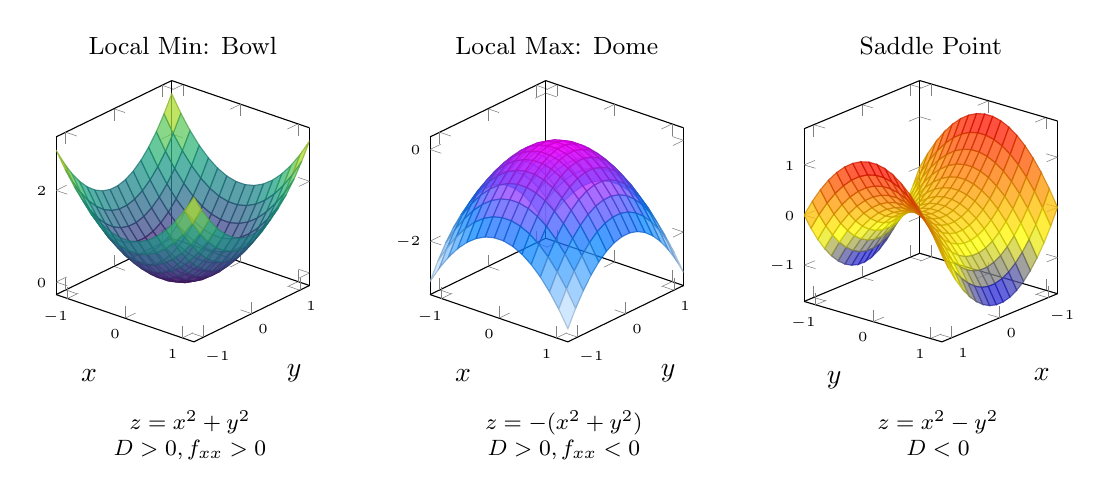
\begin{tikzpicture}
% Panel 1: Local Minimum (Bowl)
\begin{scope}[shift={(0,0)}]
\begin{axis}[
  width=4.8cm, height=4.9cm,
  view={40}{25},
  xlabel={$x$}, ylabel={$y$},
  tick label style={font=\tiny},
  domain=-1.2:1.2, y domain=-1.2:1.2,
  samples=16, samples y=16,
  title style={font=\small},
  title={Local Min: Bowl},
]
\addplot3[surf, opacity=0.75, colormap/viridis] {x^2 + y^2};
\end{axis}
\node[below, font=\footnotesize, align=center] at (1.7,-0.75) {$z=x^2+y^2$\\$D>0, f_{xx}>0$};
\end{scope}

% Panel 2: Local Maximum (Dome)
\begin{scope}[shift={(4.75,0)}]
\begin{axis}[
  width=4.8cm, height=4.9cm,
  view={40}{25},
  xlabel={$x$}, ylabel={$y$},
  tick label style={font=\tiny},
  domain=-1.2:1.2, y domain=-1.2:1.2,
  samples=16, samples y=16,
  title style={font=\small},
  title={Local Max: Dome},
]
\addplot3[surf, opacity=0.75, colormap/cool] {-(x^2 + y^2)};
\end{axis}
\node[below, font=\footnotesize, align=center] at (1.7,-0.75) {$z=-(x^2+y^2)$\\$D>0, f_{xx}<0$};
\end{scope}

% Panel 3: Saddle Point
\begin{scope}[shift={(9.5,0)}]
\begin{axis}[
  width=4.8cm, height=4.9cm,
  view={130}{20},
  xlabel={$x$}, ylabel={$y$},
  tick label style={font=\tiny},
  domain=-1.2:1.2, y domain=-1.2:1.2,
  samples=18, samples y=18,
  title style={font=\small},
  title={Saddle Point},
]
\addplot3[surf, opacity=0.75, colormap/hot] {x^2 - y^2};
\end{axis}
\node[below, font=\footnotesize, align=center] at (1.7,-0.75) {$z=x^2-y^2$\\$D<0$};
\end{scope}
\end{tikzpicture}
\caption{The three kinds of critical point in two variables, each at the origin.
Left: a local minimum ($z=x^2+y^2$), curving up in every direction.
Center: a local maximum ($z=-(x^2+y^2)$), curving down in every direction.
Right: a saddle point ($z=x^2-y^2$), curving up along the $x$-axis and down along the $y$-axis;
its tangent plane at $(0,0)$ is horizontal, yet the point is neither a peak nor a valley.
The labels $D$ and $f_{xx}$ refer to the test in the next subsection.}
\label{ch33:fig-saddle}
\end{figure}

\subsection{The second-derivative test, intuitively}

How do we tell the three apart without plotting? By looking at \emph{curvature}
(how the surface bends), which is measured by second derivatives. In one variable, after $f'(a)=0$, the sign of $f''(a)$
decided max ($f''<0$, concave down) versus min ($f''>0$, concave up). In two
variables there are \emph{three} second partials to track,
\[
  f_{xx} = \pdv{}{x}\Big(\pdv{f}{x}\Big),\qquad
  f_{yy} = \pdv{}{y}\Big(\pdv{f}{y}\Big),\qquad
  f_{xy} = \pdv{}{y}\Big(\pdv{f}{x}\Big),
\]
(and for the functions we meet, $f_{xy}=f_{yx}$, the mixed partials agree, as in
Chapter~32). A rectangular grid of numbers is called a \textbf{matrix}. We
arrange the second partials in a $2\times 2$ matrix called the \textbf{Hessian
matrix} (after Otto Hesse):
\[
  H = \begin{pmatrix} f_{xx} & f_{xy} \\ f_{xy} & f_{yy}\end{pmatrix}.
\]
The Hessian is the multivariable second derivative: it records the curvature of
the surface in every direction, just as the gradient recorded the slope in every
direction. The quantity that decides the verdict is its \textbf{determinant}. For
a $2\times2$ matrix $\begin{pmatrix} p & q\\ r & s\end{pmatrix}$ the determinant
is the single number $ps-qr$ (top-left times bottom-right, minus top-right times
bottom-left). For the Hessian it is
\[
  D = f_{xx}f_{yy} - (f_{xy})^2.
\]

\begin{focusbox}
\textbf{The second-derivative (Hessian) test.} At a critical point $(a,b)$, let
$D = f_{xx}f_{yy} - f_{xy}^2$, all evaluated at $(a,b)$.
\begin{itemize}
\item If $D>0$ and $f_{xx}>0$: \textbf{local minimum} (a bowl, curving up).
\item If $D>0$ and $f_{xx}<0$: \textbf{local maximum} (a dome, curving down).
\item If $D<0$: \textbf{saddle point} (curving up one way, down another).
\item If $D=0$: the test is \textbf{inconclusive} -- the curvature is too gentle
to decide, and other methods are needed.
\end{itemize}
\end{focusbox}

\begin{intuitionbox}
Where does $D = f_{xx}f_{yy}-f_{xy}^2$ come from? Two things must be
true for a real bowl. First, it must curve up along the $x$-direction
\emph{and} along the $y$-direction: $f_{xx}>0$ and $f_{yy}>0$. But that is not
enough -- a strong mixed term $f_{xy}$ can twist the surface so that even though
both axis-directions curve up, some diagonal direction curves \emph{down},
producing a saddle surface. The determinant $D$ catches this twist: requiring $f_{xx}f_{yy} > f_{xy}^2$ says the upward
curvature beats the twisting. When the twist wins ($D<0$), you have a saddle: up
some ways, down others. When $D>0$, the sign of $f_{xx}$ then tells bowl ($+$)
from dome ($-$). This is the two-dimensional version of ``concave up versus
concave down,'' with $D$ guarding against mixed diagonal curvature.
\end{intuitionbox}

\begin{whybox}
\textbf{Why the determinant decides it.} Near a critical point
the gradient is zero, so the linear part of $f$ vanishes and the \emph{quadratic}
part (the two-variable analogue of the term $\tfrac12 f''(a)h^2$ in the Taylor
polynomial of Chapter~31) takes over. Writing $h$ and $k$ for small steps in $x$
and $y$,
\[
  f(a+h,b+k) \approx f(a,b) + \tfrac12\big(f_{xx}h^2 + 2f_{xy}hk + f_{yy}k^2\big).
\]
The type of the critical point depends on the sign of
$Q(h,k)=f_{xx}h^2 + 2f_{xy}hk + f_{yy}k^2$, a \emph{quadratic form}: a sum of
terms of degree exactly two in $h$ and $k$. If $Q>0$ for every direction $(h,k)$,
the surface rises every way -- a min. If $Q<0$ always -- a max. If $Q$ is positive
some ways and negative others -- a saddle. Completing the square (assuming
$f_{xx}\neq 0$),
\[
  Q = f_{xx}\Big(h + \tfrac{f_{xy}}{f_{xx}}k\Big)^2
      + \frac{f_{xx}f_{yy}-f_{xy}^2}{f_{xx}}\,k^2,
\]
and you can read off everything: the leftover coefficient on $k^2$ is $D/f_{xx}$.
For $Q$ to keep one sign, both pieces need matching signs, which forces $D>0$;
then $f_{xx}$ sets that sign (min if $+$, max if $-$). If $D<0$ the two squared
pieces have opposite signs, so $Q$ takes both signs: a saddle. Up to a factor of
$-4$, $D$ is the \emph{discriminant} of $Q$ (the quantity $B^2-4AC$ from the
quadratic formula, here $B^2-4AC=4f_{xy}^2-4f_{xx}f_{yy}$), and it is the
two-variable version of the $f''$ sign test.
\end{whybox}

\begin{example}[Classifying every critical point]
\label{ch33:ex-classify}
Classify the critical points of $f(x,y)=x^3 - 3x + y^2$.

\textbf{Step 1: find them.} $f_x = 3x^2 - 3 = 3(x^2-1)$ and $f_y = 2y$. Setting
both to zero: $f_y=0$ gives $y=0$, and $f_x=0$ gives $x^2=1$, so $x=\pm 1$. Two
critical points: $(1,0)$ and $(-1,0)$.

\textbf{Step 2: second partials.} $f_{xx}=6x$, $f_{yy}=2$, $f_{xy}=0$. So
$D = f_{xx}f_{yy}-f_{xy}^2 = (6x)(2) - 0 = 12x$.

\textbf{Step 3: apply the test.}
\begin{itemize}
\item At $(1,0)$: $D = 12(1) = 12 > 0$ and $f_{xx}=6(1)=6>0$. \emph{Local
minimum.}
\item At $(-1,0)$: $D = 12(-1) = -12 < 0$. \emph{Saddle point.}
\end{itemize}
This fits the shape of $f$: in $x$ it is a cubic (one local min at $x=1$, one local
max at $x=-1$), and in $y$ it is the upward parabola $y^2$. At $x=1$ both
directions curve up -- a true bowl. At $x=-1$ the $x$-cubic curves down while the
$y$-parabola curves up: up one way, down the other, a saddle. The Hessian test
found all of this from three second derivatives.
\end{example}

\begin{example}[A clean maximum]
\label{ch33:ex-max}
Classify the critical point of $f(x,y)=4 - x^2 - y^2 + 2x$.

$f_x = -2x + 2 = 0 \Rightarrow x = 1$; $f_y = -2y = 0 \Rightarrow y = 0$. One
critical point $(1,0)$. Second partials: $f_{xx}=-2$, $f_{yy}=-2$, $f_{xy}=0$, so
$D = (-2)(-2) - 0 = 4 > 0$ with $f_{xx}=-2<0$: a \emph{local maximum}. Indeed
$f = 5-(x-1)^2 - y^2$ after completing the square, an upside-down bowl with summit
$5$ at $(1,0)$, as the test reported.
\end{example}

\section{Constrained Optimization and Lagrange Multipliers}
\label{ch33:lagrange-multipliers}

Up to this point we searched the whole $xy$-plane for summits, pits and saddles,
the points where $\grad f = \vec{0}$. In applications the inputs are often tied
together by a rule. An engineer wants the strongest beam that stays under a weight
limit; a shopper wants the most satisfaction from a fixed budget. Such a problem has
an \textbf{objective} $f(x,y)$, the quantity to make as large or as small as
possible (Chapter~17), and a \textbf{constraint}, an equation $g(x,y)=c$ that the
inputs must satisfy.

In Chapter~17 we handled constraints by substitution: solve $g(x,y)=c$ for one
variable, say $y=h(x)$, substitute to get $f(x,h(x))$, a function of $x$ alone, and
set its derivative to zero. That can fail. For a constraint like
$x^5 + x + y^5 + y = 1$ there is no formula for $y$ in terms of $x$, and even when
there is one, eliminating a variable can hide the symmetry of the problem. The
method of \emph{Lagrange multipliers} avoids substitution and uses the geometry of
gradients instead.

\subsection{The Geometry of Tangent Contours}

Picture a mountainside whose height above sea level is $f(x,y)$. If you could walk
anywhere, you would follow $\grad f$ uphill until you reached a peak where
$\grad f = \vec{0}$.

Now suppose you must stay on a fenced trail, the curve $g(x,y) = c$: you can only
walk forward or backward along it. Which point on the trail is highest?

Picture the elevation contours $f(x,y) = k$ of the mountain. As you walk along the
trail, you cross from one contour to another:
\begin{itemize}
\item Suppose that at your position the trail cuts \emph{across} the contour
$f(x,y) = k$ at an angle. Then stepping one way along the trail takes you to higher
contours ($f > k$), and stepping the other way takes you to lower ones ($f < k$).
\item So such a point cannot be the highest or lowest point of the trail. In terms
of the gradient: let $\vec{T}$ be a unit vector pointing along the trail (a
\emph{unit tangent vector}). The rate of change of $f$ as you walk along the trail
is the directional derivative $D_{\vec{T}} f = \grad f \cdot \vec{T}$, and at
such a point it is not zero. If it is positive, stepping forward climbs; if it is negative, stepping backward
climbs.
\end{itemize}

The climb can stop only where walking along the trail gives zero rate of change:
where the trail stops cutting across the contours and, for an instant, runs along
one of them. So at a constrained maximum or minimum $(x^*, y^*)$ (the star marks
the best point), the contour $f(x,y) = k^*$ through that point must be
\textbf{tangent to the constraint curve $g(x,y)=c$}: the two curves touch and share
a tangent line there. Figure~\ref{ch33:fig-lagrange-kiss} shows both situations.

\textbf{Pause and think:} If the objective is $f(x,y)=x^2+y^2$ (a bowl) and the constraint is the line $x+y=2$, what does the tangency condition look like? The level curves of $f$ are concentric circles centered at the origin. The constraint is a straight diagonal line. The lowest point on the line corresponds to the smallest circle that touches the line -- touching it tangentially at $(1,1)$.

\begin{figure}[htbp]
\centering
\begin{tikzpicture}
\begin{axis}[
  width=6.3cm, axis equal image,
  xmin=0, xmax=4.4, ymin=0, ymax=4.4,
  axis lines=left, xlabel={$x$}, ylabel={$y$},
  xtick={1,2,3,4}, ytick={1,2,3,4},
  tick label style={font=\footnotesize},
  clip=false, title style={font=\small, yshift=8pt},
  title={(a) A contour crosses the trail},
]
\addplot[targetgreen!70, thick, dashed, samples=60, domain=0.909:4.4] {4/x};
\node[targetgreen!70!black, anchor=south, font=\footnotesize] at (axis cs:0.909,4.4) {$f=4$};
\addplot[targetgreen, very thick, samples=60, domain=0.682:4.4] {3/x};
\node[targetgreen!80!black, anchor=west, font=\footnotesize] at (axis cs:4.4,0.682) {$f=3$};
\addplot[curveblue, line width=1.4pt, domain=0:4] {4-x};
\node[curveblue, font=\footnotesize, anchor=west] at (axis cs:0.1,0.35) {trail $x+y=4$};
% gradient at P=(3,1), drawn at half length: (0.5,1.5)
\draw[-{Stealth[length=2.5mm]}, tangentred, very thick] (axis cs:3,1) -- (axis cs:3.5,2.5)
  node[above, font=\footnotesize] {$\grad f$};
% unit tangent T along the trail
\draw[-{Stealth[length=2.5mm]}, sourceblue!70!black, thick] (axis cs:3,1) -- (axis cs:2.293,1.707)
  node[above right=-1pt, font=\footnotesize] {$\vec T$};
% shadow of grad f on the trail direction: (-0.5,0.5)
\draw[gray, thin, dashed] (axis cs:3.5,2.5) -- (axis cs:2.5,1.5);
\draw[quotientorange, line width=2.4pt] (axis cs:3,1) -- (axis cs:2.5,1.5);
\fill (axis cs:3,1) circle (1.8pt) node[below left, font=\footnotesize] {$P$};
\end{axis}
\begin{scope}[xshift=7.1cm]
\begin{axis}[
  width=6.3cm, axis equal image,
  xmin=0, xmax=4.4, ymin=0, ymax=4.4,
  axis lines=left, xlabel={$x$}, ylabel={$y$},
  xtick={1,2,3,4}, ytick={1,2,3,4},
  tick label style={font=\footnotesize},
  clip=false, title style={font=\small, yshift=8pt},
  title={(b) A contour touches the trail},
]
\addplot[targetgreen!70, thick, dashed, samples=60, domain=1.136:4.4] {5/x};
\node[targetgreen!70!black, anchor=west, font=\footnotesize] at (axis cs:4.4,1.136) {$f=5$};
\addplot[targetgreen, very thick, samples=60, domain=0.909:4.4] {4/x};
\node[targetgreen!80!black, anchor=south, font=\footnotesize] at (axis cs:0.909,4.4) {$f=4$};
\addplot[targetgreen!70, thick, dashed, samples=60, domain=0.682:4.4] {3/x};
\node[targetgreen!70!black, anchor=west, font=\footnotesize] at (axis cs:4.4,0.682) {$f=3$};
\addplot[curveblue, line width=1.4pt, domain=0:4] {4-x};
\node[curveblue, font=\footnotesize, anchor=west] at (axis cs:0.1,0.35) {trail $x+y=4$};
% grad f = (2,2) and grad g = (1,1) at (2,2), both at half length
\draw[-{Stealth[length=2.5mm]}, tangentred, very thick] (axis cs:2,2) -- (axis cs:3,3)
  node[right, font=\footnotesize] {$\grad f$};
\draw[-{Stealth[length=2.5mm]}, sourceblue, very thick] (axis cs:2,2) -- (axis cs:2.5,2.5)
  node[right=2pt, font=\footnotesize] {$\grad g$};
\fill (axis cs:2,2) circle (1.8pt) node[below left, font=\footnotesize] {$(2,2)$};
\end{axis}
\end{scope}
\end{tikzpicture}
\caption{Maximizing $f(x,y)=xy$ on the trail $x+y=4$ (blue line); the green curves are
contours of $f$. (a) At $P=(3,1)$ the contour $f=3$ crosses the trail. The gradient
$\grad f=(1,3)$ has a nonzero shadow (orange) on the trail direction $\vec T$, so
walking along the trail toward the upper left increases $f$. (b) At $(2,2)$ the
contour $f=4$ touches the trail without crossing it, and the contour $f=5$ is out
of reach. There $\grad f=(2,2)$ and $\grad g=(1,1)$ point along the same line:
$\grad f=2\,\grad g$. (Arrows are drawn at half length.)}
\label{ch33:fig-lagrange-kiss}
\end{figure}

Now combine this tangency with the fact from Section~\ref{ch33:perp}: \emph{wherever the gradient of a differentiable function is nonzero, it is perpendicular to the level curve through that point}.
\begin{enumerate}
\item The contour $f(x,y) = k^*$ has normal (perpendicular) vector $\grad f(x^*, y^*)$.
\item The constraint path $g(x,y) = c$ is itself a level curve of $g$, so its normal vector is $\grad g(x^*, y^*)$.
\item Because the two curves are tangent at $(x^*, y^*)$, they share the exact same tangent line.
\item Two curves in the plane that share a tangent line also share the line perpendicular to it.
\end{enumerate}

Therefore the normal vectors $\grad f(x^*, y^*)$ and $\grad g(x^*, y^*)$ point along the same line. Two vectors lie along the same line if and only if one is a scalar multiple of the other:
\begin{equation}
\grad f(x^*, y^*) = \lambda \grad g(x^*, y^*),
\label{ch33:eq-lagrange}
\end{equation}
for some number $\lambda \in \R$ (the Greek letter lambda), called the \textbf{Lagrange multiplier}. This needs $\grad g(x^*, y^*) \neq \vec{0}$; otherwise $g$ has no well-defined normal direction there. (A plain number, as opposed to a vector, is often called a \emph{scalar}.)

In two dimensions, expanding Equation~\eqref{ch33:eq-lagrange} into components yields two scalar equations:
\[
f_x(x,y) = \lambda g_x(x,y), \qquad f_y(x,y) = \lambda g_y(x,y).
\]
Together with the constraint equation $g(x,y) = c$, this gives three equations in three unknowns $x$, $y$, $\lambda$. Every candidate for a local constrained maximum or minimum must satisfy this system.

\subsection{The Physical Meaning of \texorpdfstring{$\lambda$}{lambda}: Shadow Price and Sensitivity}

The number $\lambda$ has a meaning of its own.

Suppose the constraint value $c$ (think of it as a budget) changes by a small amount $\dd c$: for instance, you are granted one more unit of money, fuel, or material. The constraint curve shifts slightly, and so does the best elevation you can reach on it. How much does the optimal value $f^*$ change per unit change in $c$?

Let $\vec{r}^*(c) = (x^*(c), y^*(c))$ denote the position of the constrained optimum as a function of the parameter $c$, and let $f^*(c) = f(\vec{r}^*(c))$ be the optimal value achieved. By the multivariable chain rule:
\[
\dv{f^*}{c} = \grad f(\vec{r}^*(c)) \cdot \dv{\vec{r}^*}{c}.
\]
At the optimum, the gradient condition holds: $\grad f = \lambda \grad g$. Substituting this into the chain rule gives:
\[
\dv{f^*}{c} = \lambda \left( \grad g(\vec{r}^*(c)) \cdot \dv{\vec{r}^*}{c} \right).
\]
Now differentiate the constraint identity $g(\vec{r}^*(c)) = c$ with respect to $c$, again applying the multivariable chain rule:
\[
\dv{}{c}\big[g(\vec{r}^*(c))\big] = \grad g(\vec{r}^*(c)) \cdot \dv{\vec{r}^*}{c} = \dv{}{c}[c] = 1.
\]
So the dot product in parentheses equals $1$, and therefore
\begin{equation}
\dv{f^*}{c} = \lambda.
\label{ch33:eq-shadow-price}
\end{equation}

The Lagrange multiplier is the rate at which the best achievable value changes as the constraint is loosened. Economists call $\lambda$ the \textbf{shadow price} of the constraint: the value of one more unit of the limited resource, and so the most you should be willing to pay for it. (``Marginal'' in economics means ``per additional unit,'' so $\lambda$ is also called the marginal value of the resource.)
\begin{itemize}
\item If $\lambda = 5$, raising the budget $c$ by $0.01$ raises the best achievable value by about $5 \times 0.01 = 0.05$.
\item If $\lambda = 0$, then $\grad f(x^*,y^*) = \vec{0}$: the optimum on the curve happens to be a critical point of $f$ itself, so nudging $c$ changes $f^*$ by zero to first order ($\dv{f^*}{c} = 0$).
\item If $\lambda$ is negative, increasing the budget parameter $c$ decreases the optimal value of $f$.
\end{itemize}
In economics and planning problems, $\lambda$ is often the number people most want to know: it says how much an extra unit of the limited resource is worth.

\subsection{Two Complete Worked Examples}

\begin{example}[Maximizing a product under a linear budget]
\label{ch33:ex-lagrange-linear}
Maximize $f(x,y) = xy$ subject to the linear constraint $g(x,y) = 2x + y = 100$, where $x, y > 0$.

\textbf{Step 1: Compute gradients.}
\[
\grad f = \begin{pmatrix} f_x \\ f_y \end{pmatrix} = \begin{pmatrix} y \\ x \end{pmatrix}, \qquad
\grad g = \begin{pmatrix} g_x \\ g_y \end{pmatrix} = \begin{pmatrix} 2 \\ 1 \end{pmatrix}.
\]

\textbf{Step 2: Set up the Lagrange system $\grad f = \lambda \grad g$.}
\begin{align}
y &= 2\lambda, \label{ch33:ex1-eq1} \\
x &= \lambda, \label{ch33:ex1-eq2} \\
2x + y &= 100. \label{ch33:ex1-eq3}
\end{align}

\textbf{Step 3: Eliminate $\lambda$ to find the optimal ratio.}
From Equation~\eqref{ch33:ex1-eq2}, $\lambda = x$. Substituting this into Equation~\eqref{ch33:ex1-eq1} gives:
\[
y = 2x.
\]
So at the optimum $f_x/f_y = y/x$ equals $g_x/g_y = 2/1$: the gains from one more unit of $x$ and of $y$ are in the same ratio as their costs in the budget.

\textbf{Step 4: Substitute into the constraint.}
Substitute $y = 2x$ into Equation~\eqref{ch33:ex1-eq3}:
\[
2x + (2x) = 100 \implies 4x = 100 \implies x^* = 25.
\]
Then $y^* = 2(25) = 50$, and the multiplier is $\lambda = x^* = 25$.

\textbf{Step 5: Compute the optimal value and verify the shadow price.}
The maximum product is:
\[
f^* = f(25, 50) = (25)(50) = 1250.
\]
To verify the physical meaning of $\lambda = 25$, consider a general budget $c$ so that $2x + y = c$. The condition $y = 2x$ remains unchanged, so $4x = c \implies x^*(c) = c/4$ and $y^*(c) = c/2$. The optimal product as a function of budget $c$ is:
\[
f^*(c) = x^*(c)\,y^*(c) = \left(\frac{c}{4}\right)\left(\frac{c}{2}\right) = \frac{c^2}{8}.
\]
Differentiating with respect to the budget $c$:
\[
\dv{f^*}{c} = \dv{}{c}\left[\frac{c^2}{8}\right] = \frac{2c}{8} = \frac{c}{4}.
\]
Evaluating at our specific budget $c = 100$:
\[
\eval{\dv{f^*}{c}}{c=100} = \frac{100}{4} = 25 = \lambda.
\]
The rate at which the optimal value increases with the budget is the Lagrange multiplier $\lambda$, as Figure~\ref{ch33:fig-shadow-price} shows.

\begin{figure}[htbp]
\centering
\begin{tikzpicture}
\begin{axis}[
  width=8.5cm, height=5.6cm,
  xmin=60, xmax=140, ymin=0, ymax=2600,
  axis lines=left,
  xlabel={budget $c$}, ylabel={best product $f^*(c)$},
  label style={font=\small}, tick label style={font=\footnotesize},
  xtick={60,80,100,120,140}, ytick={500,1250,2000},
  yticklabel style={/pgf/number format/1000 sep={,}},
  title style={font=\small}, title={$f^*(c)=c^2/8$ and its tangent at $c=100$},
]
\addplot[curveblue, very thick, samples=60, domain=60:140] {x^2/8};
\addplot[tangentred, thick, dashed, domain=70:130] {1250 + 25*(x-100)};
\addplot[only marks, mark=*, mark size=1.8pt, black] coordinates {(100,1250)};
\node[tangentred, font=\footnotesize, anchor=north west] at (axis cs:103,1250) {slope $=25=\lambda$};
\end{axis}
\end{tikzpicture}
\caption{The best product $f^*(c)=c^2/8$ as the budget $c$ varies. At $c=100$ the
tangent line (red) has slope $25$, which is the multiplier $\lambda$: one more unit
of budget buys about $25$ more units of product.}
\label{ch33:fig-shadow-price}
\end{figure}
\end{example}

\begin{example}[Quadratic forms on the unit circle: The bridge to eigenvalues]
\label{ch33:ex-lagrange-eigenvalues}
Let $a$, $b$, $c$ be numbers and maximize the quadratic form
\[
f(x,y) = a x^2 + 2b xy + c y^2
\]
subject to the unit circle constraint
\[
g(x,y) = x^2 + y^2 = 1.
\]
Linear algebra (Book~3) stores the three coefficients in a \emph{symmetric
matrix} (one that is unchanged when flipped across its main diagonal)
\[
A = \begin{pmatrix} a & b \\ b & c \end{pmatrix},
\]
and writes $\vec x=(x,y)$. The only matrix operation we need is
\emph{matrix times vector}: each row of $A$ is dotted with $\vec x$, giving
\[
A\vec x = \begin{pmatrix} ax+by \\ bx+cy \end{pmatrix}.
\]
(In that notation $f$ is written $\vec x^{T}\!A\vec x$, which means
$\vec x\cdot(A\vec x)$.)

\textbf{Step 1: Compute gradients.}
Computing the partials directly,
\[
\grad f(x,y) = \begin{pmatrix} 2ax + 2by \\ 2bx + 2cy \end{pmatrix} = 2 A \vec{x}.
\]
For the constraint $g(x,y) = x^2 + y^2$, the gradient is
\[
\grad g(x,y) = \begin{pmatrix} 2x \\ 2y \end{pmatrix} = 2\vec{x}.
\]

\textbf{Step 2: Apply the Lagrange condition $\grad f = \lambda \grad g$.}
\[
2 A \vec{x} = \lambda (2 \vec{x}) \iff A \vec{x} = \lambda \vec{x}.
\]
A vector $\vec x\neq\vec 0$ with $A\vec x=\lambda\vec x$ is called an \textbf{eigenvector} of $A$, and the number $\lambda$ is its \textbf{eigenvalue}. So the Lagrange condition for a quadratic form on the unit circle is the eigenvalue equation of linear algebra:
\begin{itemize}
\item The critical points $\vec{x}^*$ of the quadratic form on the unit circle are the \textbf{unit eigenvectors} of $A$: directions that multiplication by $A$ only stretches, without turning.
\item The Lagrange multipliers $\lambda$ are the \textbf{eigenvalues} of $A$: the stretch factors along those special directions.
\end{itemize}

\textbf{Step 3: What value does the objective attain at an eigenvector?}
Take the dot product of both sides of $A \vec{x} = \lambda \vec{x}$ with $\vec x$:
\[
f(\vec x)=\vec{x}\cdot (A \vec{x}) = \vec{x}\cdot (\lambda \vec{x}) = \lambda\, (\vec{x}\cdot \vec{x}) = \lambda\norm{\vec x}^2.
\]
Because $\vec{x}$ lies on the unit circle ($\norm{\vec{x}}^2 = 1$), this simplifies to
\[
f(\vec{x}) = \lambda.
\]
The value of the quadratic form at any critical point is the corresponding eigenvalue. Therefore:
\begin{itemize}
\item The \textbf{maximum} of $f$ on the unit circle is the largest eigenvalue $\lambda_{\max}$.
\item The \textbf{minimum} of $f$ on the unit circle is the smallest eigenvalue $\lambda_{\min}$.
\end{itemize}

\textbf{Step 4: A concrete numerical calculation.}
Let $A = \begin{pmatrix} 5 & 2 \\ 2 & 2 \end{pmatrix}$, so $f(x,y) = 5x^2 + 4xy + 2y^2$ subject to $x^2 + y^2 = 1$. The Lagrange system $A\vec{x} = \lambda\vec{x}$ becomes:
\begin{align*}
(5 - \lambda)x + 2y &= 0, \\
2x + (2 - \lambda)y &= 0.
\end{align*}
We need a solution other than $x=y=0$, since $(0,0)$ is not on the circle. A system like this has such a solution only when the determinant of its coefficient matrix is zero (if the determinant were nonzero, $x=y=0$ would be the only solution):
\[
\det \begin{pmatrix} 5 - \lambda & 2 \\ 2 & 2 - \lambda \end{pmatrix} = (5 - \lambda)(2 - \lambda) - 4 = \lambda^2 - 7\lambda + 6 = 0.
\]
Factoring gives $(\lambda - 6)(\lambda - 1) = 0$, yielding two eigenvalues: $\lambda_1 = 6$ and $\lambda_2 = 1$.
\begin{itemize}
\item For $\lambda_1 = 6$: $(5 - 6)x + 2y = 0 \implies -x + 2y = 0 \implies x = 2y$. 
Substituting into $x^2 + y^2 = 1$ gives $(2y)^2 + y^2 = 5y^2 = 1$, so $y = \pm 1/\sqrt{5}$ and $x = \pm 2/\sqrt{5}$. 
The maximum value of $f(x,y)$ on the circle is $f^* = \lambda_1 = 6$.
\item For $\lambda_2 = 1$: $(5 - 1)x + 2y = 0 \implies 4x + 2y = 0 \implies y = -2x$. 
Substituting into $x^2 + y^2 = 1$ gives $x^2 + (-2x)^2 = 5x^2 = 1$, so $x = \pm 1/\sqrt{5}$ and $y = \mp 2/\sqrt{5}$. 
The minimum value of $f(x,y)$ on the circle is $f^* = \lambda_2 = 1$.
\end{itemize}
This links multivariable calculus to Book~3 (\emph{Linear Algebra From the Ground Up}). There, the \emph{principal axis theorem} says that every symmetric matrix stretches the plane along two perpendicular directions; here those directions are $(2,1)$ and $(1,-2)$ (up to length), found as the maximum and minimum of a constrained optimization problem.
\end{example}

\begin{historybox}
The tools in this chapter came from physics and astronomy. In 1788, Joseph-Louis Lagrange sought a way to calculate the motion of pendulums and other bodies forced to move along curved tracks, without having to compute the forces the tracks exert. His method of multipliers relied on a geometric observation: because constraint forces act normal to the constraint surface, the objective gradient and constraint gradient must align along a shared normal line, $\grad f = \lambda \grad g$.

In 1847, two key developments appeared. In Paris, Augustin-Louis Cauchy computed planetary orbits by taking iterative steps downhill in the direction of steepest descent, introducing gradient descent. In Dublin, around the same time, William Rowan Hamilton introduced an early form of the symbol $\grad$ while developing quaternions (a four-dimensional number system that extends the complex numbers). The name \emph{nabla} was suggested to Peter Guthrie Tait because the symbol resembled an ancient Hebrew harp.

In the 1880s and 1890s, Josiah Willard Gibbs and Oliver Heaviside extracted the dot product, the cross product and the gradient from quaternions to build modern vector calculus, which gave a compact form to Maxwell's equations of electricity and magnetism. Earlier, in the 1840s, Otto Hesse had organized second partial derivatives into the Hessian matrix to classify local curvature.

Open questions remain. For loss surfaces with many valleys and saddles in millions of dimensions (as in neural networks), understanding when and why gradient descent avoids saddle points and settles into good local minima is an active research area.
\end{historybox}

\begin{recoverybox}
The chapter in six statements. (1) The
\emph{directional derivative} $D_{\vec u}f$ is the slope of $f$ as you walk in the
unit direction $\vec u$, and it equals $\grad f\cdot\vec u$. (2) The
\emph{gradient} $\grad f = (f_x,f_y)$ points in the direction of steepest ascent,
its length is the steepest slope, and it is perpendicular to level curves. (3) The
\emph{chain rule} ``multiply along paths, add across paths'' computes derivatives
through any chain of dependencies and is what backpropagation uses. (4) Linear
approximation upgrades the tangent line to a tangent \emph{plane},
$L = f(a,b) + \grad f\cdot((x,y)-(a,b))$. (5) Unconstrained critical points are where
$\grad f = \vec 0$, classified by the \emph{Hessian} determinant $D=f_{xx}f_{yy}-f_{xy}^2$.
(6) Constrained extrema occur where the objective contour is tangent to the constraint path,
aligning their perpendicular gradients: $\grad f = \lambda \grad g$, where $\lambda = \dv{f^*}{c}$
measures the shadow price of the budget.
\end{recoverybox}

\begin{connectionbox}
\textbf{Looking ahead: from local slopes to global volume.}
Chapters~32 and~33 built the differential half of multivariable calculus: zoom in on a point until the surface looks like a flat plane, and read off its slopes from $\grad f$.
Chapter~34 builds the other half: chop a region or solid into tiny cells, add up a function over all of them, and recover volume, mass, and probability -- the two-dimensional version of the Riemann sum.
\end{connectionbox}

\section{Exercises}
\label{ch33:exercises}

\begin{exercise}[Directional derivative, by formula]
\label{ch33:exr-dir}
Let $f(x,y) = x^2 y + y^3$. Compute the directional derivative of $f$ at the point
$(2,1)$ in the direction toward $(5,5)$. (Remember to normalize the direction
vector first.)
\end{exercise}

\begin{exercise}[Steepest ascent]
\label{ch33:exr-steep}
For $f(x,y) = e^{x}\sin y$, find at the point $(0,\tfrac{\pi}{2})$: (a) the
gradient, (b) the unit direction of steepest ascent, and (c) the maximum rate of
increase. In what direction(s) is the directional derivative zero?
\end{exercise}

\begin{exercise}[Chain rule, one parameter]
\label{ch33:exr-chain1}
Let $z = x^2 - y^2$ with $x(t) = \cos t$ and $y(t) = \sin t$. Use the chain rule to
find $\dv{z}{t}$, then verify your answer by first substituting to get $z$ as an
explicit function of $t$ and differentiating directly. (You should find a clean
trigonometric expression.)
\end{exercise}

\begin{exercise}[Chain rule, two parameters]
\label{ch33:exr-chain2}
Let $z = x y$ where $x = s + t$ and $y = s - t$. Compute $\pdv{z}{s}$ and
$\pdv{z}{t}$ using the multivariable chain rule. Then compute $z$ directly in terms
of $s,t$ and confirm.
\end{exercise}

\begin{exercise}[Tangent plane and estimation]
\label{ch33:exr-plane}
Let $f(x,y) = \ln(x^2 + y^2)$. (a) Write the equation of the tangent plane to the
graph at $(1,0)$. (b) Use it to estimate $f(1.1,\,0.05)$, and compare with the true
value.
\end{exercise}

\begin{exercise}[A gradient descent run]
\label{ch33:exr-gd}
Consider $L(w_1,w_2) = w_1^2 + 4w_2^2$ with learning rate $\eta = 0.1$, starting at
$(w_1,w_2)=(1,1)$. (a) Carry out two steps of gradient descent by hand, reporting
the iterates and the loss at each. (b) Each coordinate is multiplied by a constant
factor every step -- find the two factors. Why does $w_2$ converge faster than
$w_1$, and what does that say about choosing $\eta$ when the bowl is stretched?
\end{exercise}

\begin{exercise}[Classify the critical points]
\label{ch33:exr-classify}
Find and classify all critical points of $f(x,y) = x^3 + y^3 - 3xy$ using the
Hessian test. (You should find one saddle and one local extremum.)
\end{exercise}

\begin{exercise}[The perpendicularity, concretely]
\label{ch33:exr-perp}
Let $f(x,y) = x^2 + 4y^2$, whose level curves are ellipses. At the point
$(2,1)$ (which lies on the level curve $f=8$): (a) compute $\grad f(2,1)$;
(b) find a vector tangent to the ellipse $f=8$ at $(2,1)$ (hint: parametrize, or
use implicit differentiation $\dv{y}{x}$ on $x^2+4y^2=8$); (c) verify by a dot
product that the gradient and the tangent are perpendicular.
\end{exercise}

\begin{exercise}[Conceptual: partials exist but no plane]
\label{ch33:exr-concept}
Explain in your own words, using the caution in
Section~\ref{ch33:chain}, why ``all partial derivatives exist at a point'' is
\emph{not} enough to guarantee that the chain rule formula holds there. What
stronger condition (stated in Section~\ref{ch33:tangentplane}) is the right one,
and what does it say geometrically?
\end{exercise}

\begin{exercise}[Proof: steepest ascent]
\label{ch33:exr-proof}
Prove that among all unit vectors $\vec u$, the directional derivative
$D_{\vec u} f = \grad f \cdot \vec u$ is maximized when $\vec u$ points along
$\grad f$, and that the maximum value is $\norm{\grad f}$. (Use the
identity $\grad f \cdot \vec u = \norm{\grad f}\cos\theta$ and explain why
$\cos\theta = 1$ is forced. State clearly where you use $\norm{\vec u} = 1$.)
\end{exercise}

\begin{exercise}[Proof: gradient perpendicular to level sets]
\label{ch33:exr-proofperp}
Suppose a differentiable path $\vec r(t) = (x(t), y(t))$ lies entirely on the level
curve $f(x,y) = c$. Differentiate the identity $f(x(t),y(t)) = c$ with respect to
$t$ and use the chain rule to conclude that $\grad f \cdot \vec r\,'(t) = 0$.
Explain in one sentence why this proves $\grad f$ is perpendicular to the level
curve.
\end{exercise}

\begin{exercise}[Lagrange multipliers on a circle]
\label{ch33:exr-lagrange-circle}
Find the maximum and minimum values of the linear objective $f(x,y) = x + 2y$ subject to the circular constraint $x^2 + y^2 = 5$.
\begin{enumerate}[label=(\alph*)]
  \item Set up the Lagrange system $\grad f = \lambda \grad g$ and solve for the critical points $(x,y)$ and multipliers $\lambda$.
  \item Calculate the maximum and minimum values $f^*$.
  \item Describe the geometric picture: what do the level lines $x+2y=c$ look like, and where are they tangent to the circle?
\end{enumerate}
\end{exercise}

\begin{exercise}[Mental check: shadow price in production]
\label{ch33:exr-shadow-price}
A factory produces output $P(x,y)$ from labor $x$ and capital $y$ subject to a total budget constraint $20x + 50y = B$. At the current budget $B=\$10{,}000$, the manager optimizes production using Lagrange multipliers and finds $\lambda = 1.4$.
\begin{enumerate}[label=(\alph*)]
  \item Using the identity $\dv{P^*}{B} = \lambda$, estimate the increase in maximum production if the company increases its budget by $\Delta B = \$500$.
  \item What would $\lambda = 0$ have implied about the budget constraint?
\end{enumerate}
\end{exercise}
